\begin{center}
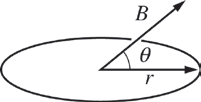
\includegraphics[scale=0.5]{images/img-003-005.png}
\end{center}

% Multiple Choice Question 6
\begin{questions}\setcounter{question}{5}\question
A circular loop of radius $r$ is located in a uniform magnetic field of magnitude $B$ directed at an angle $\theta$ to the plane of the loop, as shown above. What is the magnetic flux through the loop?

\begin{oneparchoices}
\choice $\pi r^{2} B \sin \theta$
\choice $\pi r^{2} B \cos \theta$
\choice $\pi r^{2} B$
\choice $2 \pi r B \cos \theta$
\choice $2 \pi r B$
\end{oneparchoices}\end{questions}

